\section{Selección de data (activos, frecuencia)}

Los datos para pruebas y experimentos se descargaron desde la plataforma
Dukascopy. Incialmente las pruebas se realizaron con datos a frecuencia de 1
minuto, pero luego se implementó en clase Reader los métodos correspondientes
para manejar la data ticks de forma automática: juntar datos de distintas monedas
(Bid o Ask), hacer un resampling a diferentes frecuencias, normalizar las
monedas dejando siempre la misma base, etc.

Los ticks están compuestos por: \emph{Date}, \emph{Time}, \emph{Ask},
\emph{Bid}, \emph{AskVolume}, \emph{BidVolume}. Por ser datos ticks, el campo
Time es un hora \emph{double}, es decir, tiene asociada una
hora:minutos:segundos, donde segundos es un número no entero. Cabe destacar que
no existe una clara relación entre la aparición de ticks, ya que en algunos
casos aparecen hasta 4 ticks en 1 segundo, mientras que en otros horarios no
aparecen ticks en 90 segundos (dato calculado con la función
check\_min\_frequency de la clase Reader). 

En la figura \ref{fig:eurusd_ticks} se puede apreciar la data ticks del EURUSD,
en una ventana de 30 minutos, donde la curva superior es la correspondiente al
Ask, y la inferior al Bid. En la figura \ref{fig:eurusd_r6s} se muestra la
misma moneda pero con un resample de 6 segundos. El resample se calcula con el
promedio de los ticks en la ventana de 6 segundos, y para el caso que no exista
movimiento en dicho periodo, se rellena con el valor anteior.

\begin{figure}[h!t]
    \begin{center}
        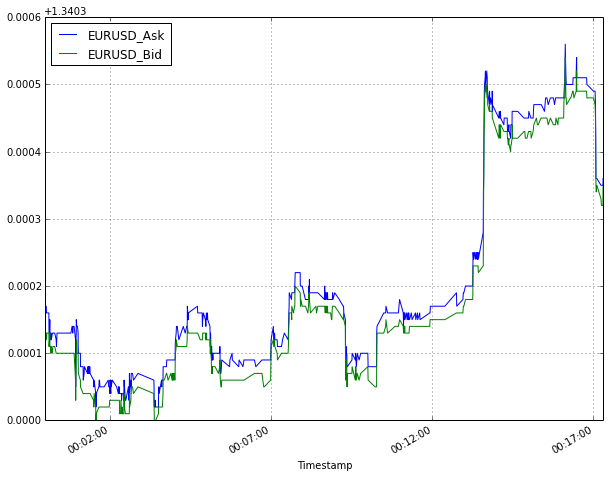
\includegraphics[width=0.6\textwidth]{images/eurusd}
        \caption{Ticks de EURUSD, Ventana de 30 minutos}
        \label{fig:eurusd_ticks}
    \end{center}
\end{figure}

\begin{figure}[h!t]
    \begin{center}
        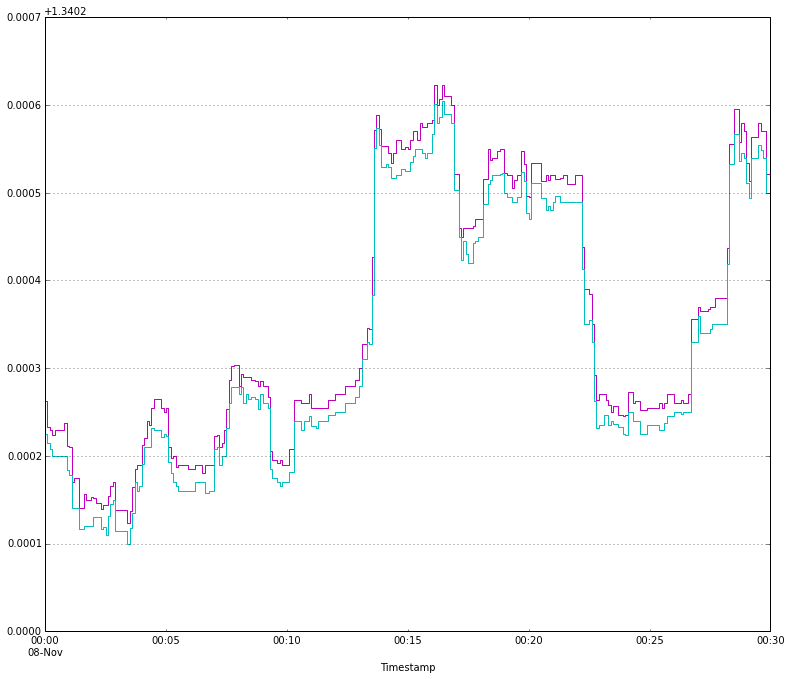
\includegraphics[width=0.6\textwidth]{images/eurusd_6s}
        \caption{Ticks de EURUSD con resample de 6 segundos}
        \label{fig:eurusd_r6s}
    \end{center}
\end{figure}

\newpage
\section{Parámetros del algoritmo}
Cómo se puede desprender de la formulación matemática de los modelos, hay dos
parámetros que deben ser definidos: largo de la ventana (L), cantidad de lags
(P). Existen variados métodos para la estimación de parámetros, sin embargo se
usará el criterio de información de Akaike Information Criterion.

\subsection{Criterio de información de Akaike}
El Criterio de información de Akaike (AIC por sus siglas en inglés) fue
inicialmente desarrollado en series temporales \emph{citar}. Su idea clave es
la de penalizar un exceso de parámetros ajustados para cierto modelo. El AIC es
un estimador muestral de $E[ln(f(X|\theta)]$, esperanza de la log-verisimilitud
(o negantropìa) que viene dado por la expresión~\ref{eq:aicformula}:

\begin{equation}
\label{eq:aicformula}
AIC = \underset{\text{bias}}{-\frac{2l}{N}} + 
\underset{\text{variance}}{\frac{2k}{N}}
\end{equation}

\noindent donde

\begin{description}
\item[l] es la función verosimilitud
\item[k] número de parámetros ajustados (incluyendo la varinza)
\item[N] número de observaciones
\end{description}

Se calcula el valor de AIC para cada modelo con el mismo set de datos, y
el \emph{mejor} modelo es el que tiene menor valor de AIC.
El primer término de AIC puede ser interpretado como una medida de la bondad
del ajuste, mientras el segundo término es una penalización, creciente conforme
aumenta el número de parámetros, de acuerdo al Principio de
Parsimonia~\ref{fig:parsimony}. El AIC enfatiza la bondad del modelo, sin
embargo no pretende identificar el modelo verdadero. Que un modelo sea el que
mejor ajusta a los datos, no quiere decir que sea el modelo real o verdadero.
Más bien, significa que el modelo es el mejor entre los modelos candidatos, en
el sentido que proporciona la aproximación más cercana a la realidad o al
verdadero modelo. El modelo que mejor se ajusta a los datos, podría cambiar
mucho en función del tamaño muestral, como en el caso de los polinomios
interpoladores. 

\begin{figure}[h!t]
    \begin{center}
        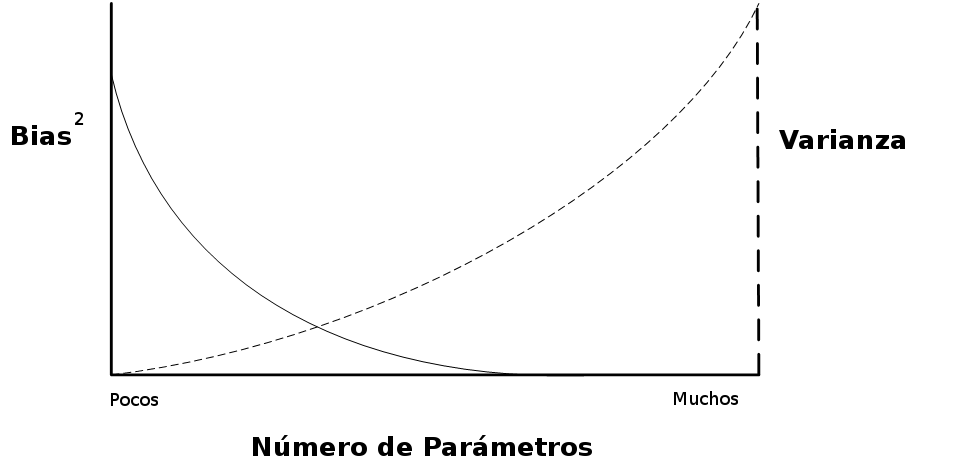
\includegraphics[width=0.8\textwidth]{images/parsimony}
        \caption{Principio de Parsimonia}
        \label{fig:parsimony}
    \end{center}
\end{figure}

Algunas de las ventajas del AIC que lo hacen tan utilizado en la práctica, son
su simplicidad (no requiere acudir a ninguna tabla para observar el valor
correspondiente) y facilidad para ser implementado, y el hecho de que no existe
el problema de especificar subjetivamente un nivel de significación arbitrario
para contrastar dos modelos.


\section{Resultados}

\section{Performance}

